%%%%%%%%%%%%%%%%%%%%%%%%%%%%%%%%%%%%%%%%%%%%%%%%%%%%%%%%%%%%%%%%%%%%
% Overivew
%%%%%%%%%%%%%%%%%%%%%%%%%%%%%%%%%%%%%%%%%%%%%%%%%%%%%%%%%%%%%%%%%%%%

\section{Conclusion}
\label{sec:conclusion}
\begin{figure}[!t]
	\centering
	%\vspace*{-3.5mm}
	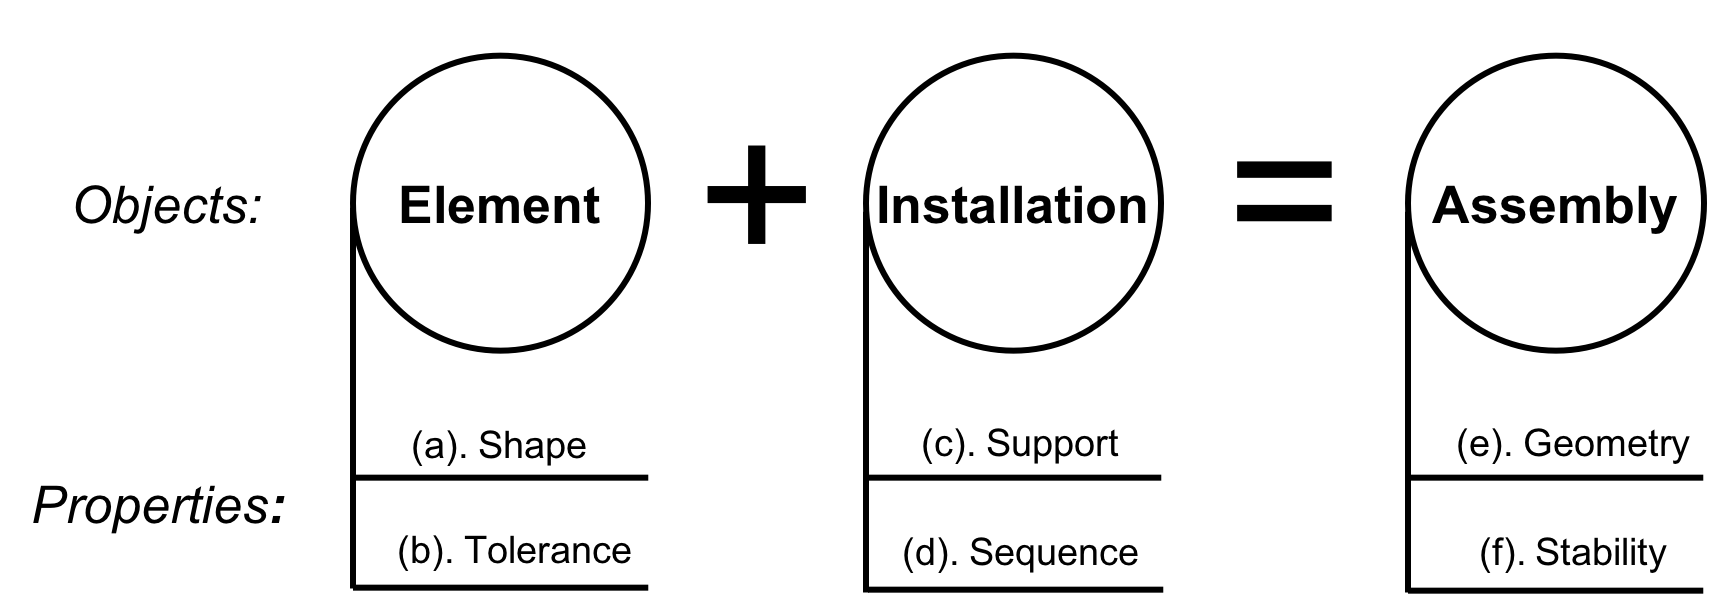
\includegraphics[width=8.00cm]{images/general_assembly.png}
	\vspace*{-2.5mm}
	\caption{The general framework of designing an assembly structure. The {\bf element} is the component part of the assembly and the {\bf installation} is the assembling process. (a) The feasible shape of element varies for different fabrication tools. For instance, 2D laser cutter only cuts 2D pattern on a flat plate but 3D printer could fabricate more freeform model. (b) Tolerance is the displacement between the fabrication and virtual model.  Machine cannot have infinite precision and the tolerance is inevitable during manufacture. (c) Temporary support such as scaffold stabilise the structure during assembling process. Less support could reduce the waste, which may takes up to 1/3 of the whole cost. (d) The assembling sequences includes the order of parts and the trajectory of placing the part in right positions. (e) User defined target geometry (f) Structural stability cares whether the whole structure will collapse under external load.
	}
	\vspace*{-4.0mm}
	\label{fig:general_assembly}
\end{figure}

This report takes a specific kind of assembly, the interlocking assembly, as an example. The interlocking property is formulated as a graph-based representation. Testing interlocking then is equivalent to analysing the strongly connected component of each DBG. The next step would be generating general interlocking structure with the help of DBGs.

However, it is better to consider more general topic beyond interlocking. The final goal of my PhD research is to build a general framework for assembly design. The composition of an general assembly includes six properties (see Fig. \ref{fig:general_assembly}). Among them, fabrication tolerance and structural stability are hard constraints and the reset have to optimize according to the demand. Besides, the framework also needs to maintain a sufficient design freedom for users. Considering all properties at same time is extremely challenging and most of the published work try to take a few properties into account. 

\vspace*{2mm}
\noindent
{\bf Properties (a) +  (d) + (e):} Most of the interlocking paper \cite{Song-2012-InterCubes},\cite{Xin-2011-BurrPuzzles}, \cite{Song-2016-CoFiFab}, \cite{Fu-2015-Furniture} are belong to this category. The constraints of installation sequence, where the key part is always the last pieces of the installation, is guaranteed by the element's shape. One of the common problem of these works is that without computing structural stability, the interlocking design is unsafe to be used in practice. Interlocking furniture, for instance, have three types of connections (see Fig.\ref{fig:Joints}). In practice, the structural strength of dovetail joint is weaker than the tenon joint. How to choose suitable joints according to the force flow while maintaining the interlocking property could be a promising research topic.
\begin{figure}[!t]
	\centering
	\vspace*{-4.0mm}
	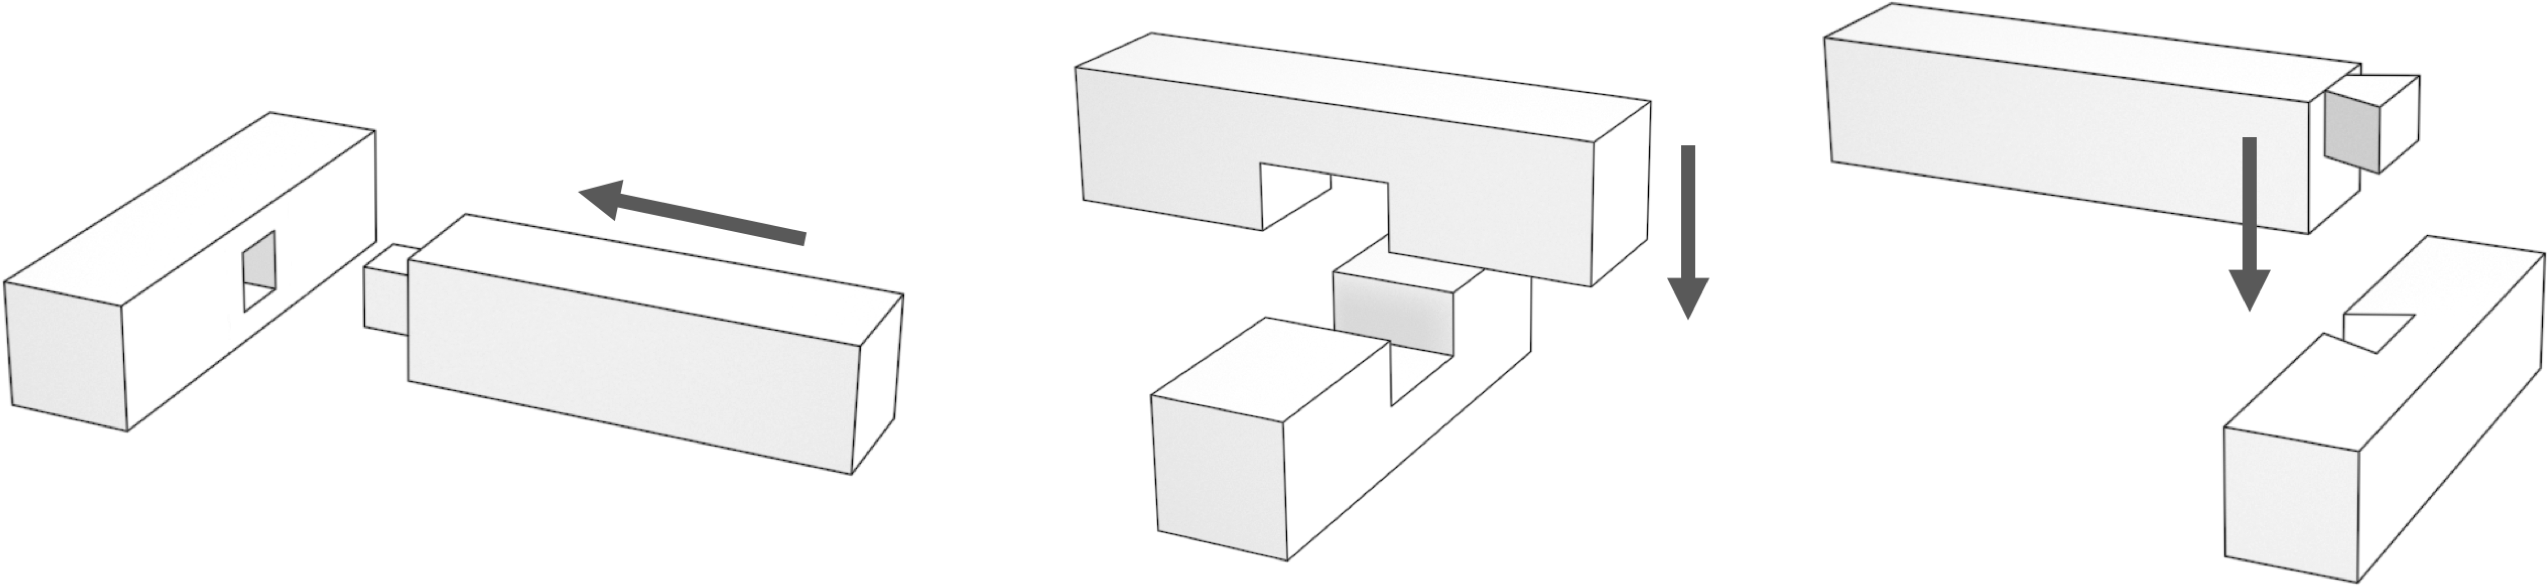
\includegraphics[width=8.00cm]{images/Joints.png}
	\vspace*{-2.5mm}
	\caption{Example woodworking joints. From left to right: mortise-and-tenon, halved joint, and dovetail joint, where the black arrow shows the single part movable direction allowed by the joint.}
	%\vspace*{-4.0mm}
	\label{fig:Joints}
\end{figure}

\vspace*{2mm}
\noindent
{\bf Properties (a) + (b) + (e):} Tolerance are usually required to accommodate the engineering error during manufacture, this resulted empty space allows each part of the assembly to have a small displacement. The accumulation of these displacements could be amplified greatly in a not well design and severely undermine the structure's stability (see Fig.\ref{fig:Gap_Issue}). A survey work of tolerance analysis is presented in \cite{chen2014comprehensive}. The tolerance analysis in mechanical engineering often deals with simple geometry and clear accumulation mechanism. However, our objects usually have complicated surface with ambiguous tolerance accumulation mechanism. One possible approach is to find the connection between the tolerance accumulation and cycles in DBGs. 
\begin{figure}[!b]
	\centering
	\vspace*{-3.0mm}
	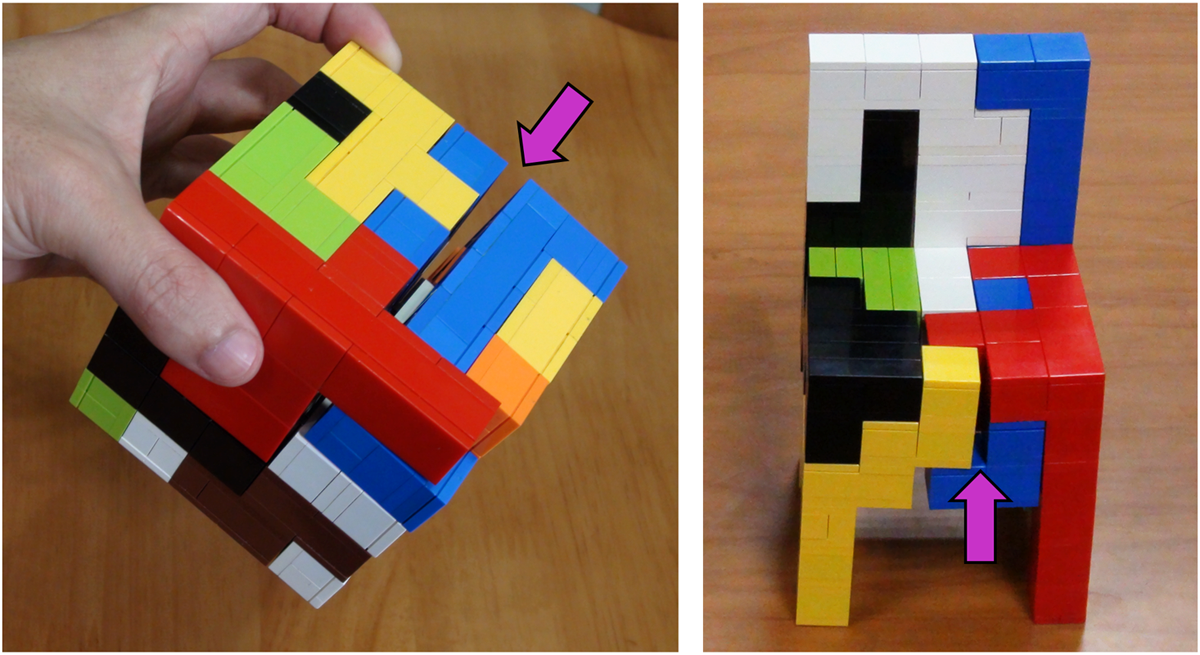
\includegraphics[width=8.30cm]{images/Gap_Issue.png}
	\vspace*{-1.0mm}
	\caption{Two  interlocking  puzzles  designed  by  implementing \cite{Song-2012-InterCubes}:  a  13-piece  cube  (left)  and  a  6-piece  chair  (right). Although being interlocking, both puzzles have the problematic gap issue (see arrows above) that loosens their structures. Note: LEGO bricks in fact have a tolerance of 0.20mm.
	}
	\vspace*{-4.5mm}
	\label{fig:Gap_Issue}
\end{figure}